\section{Commercial and Currency Integration}\label{sec:commercial}
In previous section we discussed the economic theory when a group of countries should share a currency.
Those conditions do not explain what exactly happened in the European Union where all six countries we study belong to the single market.
Labor and capital can move freely between each other country and the euro area.
Although most of the six countries we study look like suitable candidates for adoption.
They have not adopted the euro and the reason are legal and political more than economic.
We will discuss how each currency has been managed since 2005 and how they are different from each other.

\vspace{\baselineskip}

\begin{figure}[htbp]
\centering
\hyphenpenalty=10000 \exhyphenpenalty=10000
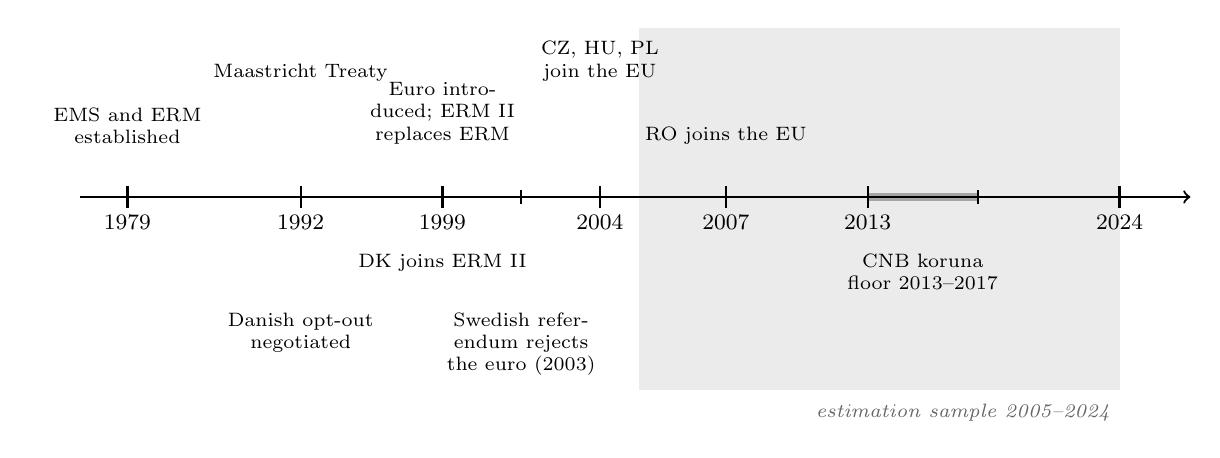
\begin{tikzpicture}[x=1.0cm, y=1cm]
% estimation window
\fill[black!8] (6.5,-2.45) rectangle (12.6,2.15);
\node[font=\scriptsize\itshape, black!60, anchor=north east] at (12.6,-2.5)
  {estimation sample 2005--2024};
% koruna floor span
\draw[line width=3pt, black!35] (9.4,0) -- (10.8,0);
% axis
\draw[->, thick] (-0.6,0) -- (13.5,0);
% ticks and years
\foreach \x/\lab in {0/1979, 2.2/1992, 4.0/1999, 6.0/2004, 7.6/2007, 9.4/2013, 12.6/2024}
  {\draw[thick] (\x,-0.14) -- (\x,0.14);
   \node[font=\footnotesize, below=3pt] at (\x,0) {\lab};}
\draw[thick] (5.0,-0.09) -- (5.0,0.09);
\draw[thick] (10.8,-0.09) -- (10.8,0.09);
% euro area institutions, above the line
\node[font=\scriptsize, align=center, anchor=south, text width=2.3cm] at (0,0.55)
  {EMS and ERM established};
\node[font=\scriptsize, align=center, anchor=south, text width=2.3cm] at (2.2,1.35)
  {Maastricht Treaty};
\node[font=\scriptsize, align=center, anchor=south, text width=2.5cm] at (4.0,0.55)
  {Euro introduced; ERM~II replaces ERM};
\node[font=\scriptsize, align=center, anchor=south, text width=2.3cm] at (6.0,1.35)
  {CZ, HU, PL join the EU};
\node[font=\scriptsize, align=center, anchor=south, text width=2.3cm] at (7.6,0.55)
  {RO joins the EU};
% national currency decisions, below the line
\node[font=\scriptsize, align=center, anchor=north, text width=2.3cm] at (2.2,-1.35)
  {Danish opt-out negotiated};
\node[font=\scriptsize, align=center, anchor=north, text width=2.3cm] at (4.0,-0.6)
  {DK joins ERM~II};
\node[font=\scriptsize, align=center, anchor=north, text width=2.5cm] at (5.0,-1.35)
  {Swedish referendum rejects the euro (2003)};
\node[font=\scriptsize, align=center, anchor=north, text width=2.6cm] at (10.1,-0.6)
  {CNB koruna floor 2013--2017};
% row labels

\end{tikzpicture}
\caption{Calendar of European monetary integration and the estimation window (2005--2024).}
\label{fig:timeline}
\end{figure}

Before turning to the main point, it is worth setting out the historical background and the conditions for joining the euro.
The monetary European Monetary was set up in 1979 to keep the exchange rate stable between members and encourage central banks working together (\cite{council_of_the_european_union_joining_2026}).
Currencies were kept within the agreed limits through Exchange Rate Mechanism.
Mutual agreement can change the rates which meant states gave up controls over their own currencies.
This system ended in 1999 when euro is introduced and the monetary policy passed to European Central Bank.
ERM II replaced the old mechanism which use as the framework for countries preparing to adopt the euro.

\vspace{\baselineskip}
\begin{table}[htbp]
\centering\small
\caption{Convergence criteria and the position of the six non-euro member states.}
\label{tab:convergence}
\begin{tabular}{L{2.4cm} L{4.2cm} c c c c c c}
\toprule
\multirow{2}{*}{\textbf{Criterion}} & \multirow{2}{*}{\textbf{Reference value}} & \multicolumn{6}{c}{\textbf{Fulfilled (2024)}} \\
\cmidrule(l){3-8}
 &  & CZ & DK & HU & PL & RO & SE \\
\midrule
Price stability & Inflation $\leq$ 1.5 pp above the three best performers & \emph{verify} & \emph{verify} & \emph{verify} & \emph{verify} & \emph{verify} & Yes \\
\addlinespace
Public finances & Deficit $<$ 3\% of GDP and debt $<$ 60\% of GDP & \emph{verify} & \emph{verify} & \emph{verify} & \emph{verify} & \emph{verify} & Yes \\
\addlinespace
Long-term interest rate & $\leq$ 2 pp above the three best performers & Yes & \emph{verify} & \emph{verify} & \emph{verify} & \emph{verify} & Yes \\
\addlinespace
Exchange rate stability & At least two years in ERM~II & No & Yes & No & No & No & No \\
\midrule
\multicolumn{2}{l}{Treaty obligation to adopt the euro} & Yes & No (opt-out) & Yes & Yes & Yes & Yes \\
\multicolumn{2}{l}{Public support for adoption (\%)} & 49 & \emph{verify} & \emph{verify} & 47 & \emph{verify} & \emph{verify} \\
\bottomrule
\end{tabular}
\caption*{\footnotesize Source: European Commission (2024) Convergence Report; Council of the European Union (2026).}
\end{table}
There are four conditions known as convergence criteria which a country must meet before adopt the euro.
It includes stable exchange rates where their inflation must be no more than 1.5 percentage points above the average of the top performing members.
The country needs stable public finances and sustainable interest rate. 
It government deficit must less than three percentage points of their GDP and its debt below 60 per cent.
And the long-term interest rates must be within two percentage points.
A country must spend at least two years in ERM II keeping its central rate close against the euro.
This condition matter more than others. This means a country can avoid adopting the euro by not joining ERM II.
And in this situation other three conditions do not matter.
Denmark is the exception case. It negotiated an opt-out from the treaties and do not required to adopt the euro.

\vspace{\baselineskip}

The six countries are outside of the euro area for different reasons. 
The Czech Republic, Hungry, Poland and Romania can be consider in one group.
None of four countries have joined ERM II.
The reason can be differ by countries and changed over time.
Most of them failed to meet the economic convergence criteria which including fiscal and inflation condition.
Out of the four countries only Czech Republic fulfilled the long-term interest rate criteria til 2024 (\cite{european_commission_european_2024}).
In the same report shows some countries lack of domestic political support.
Where Poland and Czech Republic are the lowest from six countries with 47 percentage and 49 percentage respectively.
Sweden fulfills all three condition except joining ERM II.
But the main reason it is the 2003 Referendum which Swedish public firmly voted against adopting euro with 56 percentage.
Denmark is the special case which they negotiated an exemption at Masstricht and they do not have obligation to adopt the euro.
They take part in ERM II and Danish krone close to fixed rate against the euro where central bank buy and sell to maintain it.

\vspace{\baselineskip}

The six countries managed their currencies in different ways and the differences are what make the comparison possible.
This was throughout the period we are studying from 2005 to 2024.
The Danish krone was closed to fixed rate against the euro for the whole period.
The krone barely move against the euro and it estimated volatility over the period is only a small fraction of the other countries.
The other five currencies floated but not in the same way.
The Czech National Bank operated currency floor regime against the euro from 2013 to 2017.
It prevented the koruna from strengthening beyond a stated level. 
This matter for the estimation.
The koruna was floating for part of the period and is held fixed til the end of the period.
It estimated persistence over the full sample sits close to the limit of what the model can do.
And the Romanian leu shows the same pattern for different reason.
Romanian leu is generally operating a managed float with central bank intervening more that its close countries.
The Sweden, Poland and Hungary currencies are floated and no comparable intervention.

\vspace{\baselineskip}

The six economics show differences in how much they trade with euro are same way as they manage their currencies.
Trade intensity means exports and imports measured as a share of GDP from the twenty euro area members.
Over the period it goes average from about 26 per cent in Denmark and 28 per cent in Sweden, to 37 per cent in Romania and 47 per cent in Poland, up to 85 per cent in Hungary and 88 in Czech Republic.
Czech Republic and Hungry are closely tied into German manufacturing where parts cross their borders many times before its sold.
Denmark and Sweden majorly trade with a wider set of partners where the United Kingdom and United States.
They have less of their trade in the euro.
Poland and Romania in between where they trade with euro area but their domestic economics are larger compare to the trades.

\vspace{\baselineskip}

The regime differences described above are not only the background.
It is worth to point out before the result are presented.
The exchange rate flexibility and trade exposure show different directions than the theory.
Denmark has the most fixed managed currency and the least euro are trade.
Opposite the Czech Republic and Hungry have freely floating currencies and the most euro trade.
McKinnon (\citeyear{mckinnon_optimum_1963}) shows the case more of a country trade with euro are the less its own currency is worth keeping.
The six countries show the opposite of what theory suggests which is why the interaction between volatility and trade is worth testing.

\vspace{\baselineskip}
All six of countries kept their own currencies for the whole study period.
Some studies grouped the countries by region often including the countries did adopt the euro and mixing the countries with and without their own exchange rate.
Morina et al. (\citeyear{morina_effect_2020}) report adoption was negative for growth over their period.
That is important because a sample containing countries with both sides cannot easily separate the effect of exchange rate volatility from the effect of joining the euro.
That is why the sample in this paper is on the same side.

\vspace{\baselineskip}

These currencies in sample except Danish krone are not permanently more volatile than the euro.
They are only volatile at certain periods.
Janus and Riera-Crichton (\citeyear{thorsten_pdf_2015}) find that the Great Recession raised volatility in the non-euro European countries by between 38 and 189 percentage of the sample mean.
The independent variable is the exchange rate volatility and regression can only find an effect where the variable moves.
When volatility is similar across these countries in calm periods and diverges during crises then the differences the model has to work with mostly from small number of years.
The relationship between volatility and growth should be easily show up in these years and hard to find in others.
We should consider it affects how weak result outside crisis periods meaning no relationship in calm periods.
This could also mean volatility are moving too little in the periods for a relationship to show up.
Two cannot easily be separated and we will discuss this later in the paper.
